\documentclass[convert = false, tikz]{standalone}
\usepackage[utf8]{inputenc}
\usepackage{tikz}
\usetikzlibrary{automata, positioning, arrows}
 
\usepackage{../../../../style_automata}

% arara: pdflatex
% arara: latexmk: { clean: partial }
\begin{document}
    \tikzset{
    node distance=2cm, % specifies the minimum distance between two nodes.
    }
    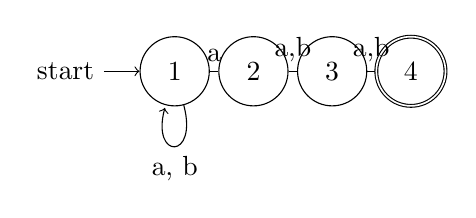
\begin{tikzpicture}
        \node[state, initial] (s0) {$1$};
        \node[state, right of=s0] (s1) {$2$};
        \node[state, right of=s1] (s2) {$3$};
        \node[state, accepting, right of=s2] (s3) {$4$};
        \draw (s0) edge[above] node{a} (s1)
        (s1) edge[above] node{a,b} (s2)
        (s2) edge[above] node{a,b} (s3)
        (s0) edge[loop below] node{a, b} (s0);
    \end{tikzpicture}
\end{document}